\documentclass[a4paper,landscape, 12pt]{article}

\usepackage[left = 2cm, bottom = 3cm, right = 3cm, top = 3cm]{geometry}
\usepackage{pgfplots}

\pagestyle{empty}

\begin{document}
\begin{figure}
    \centering
    \large

    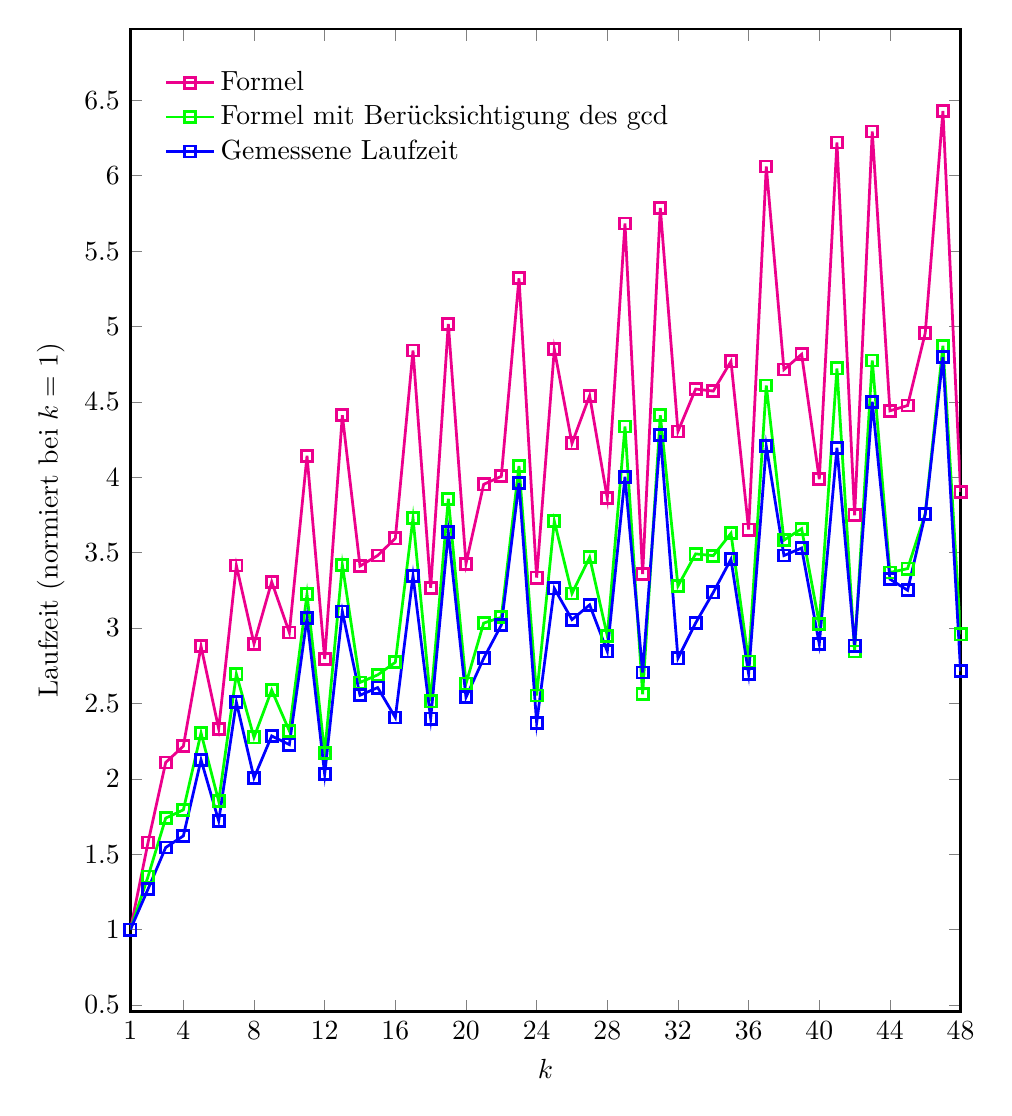
\begin{tikzpicture}
        \begin{axis}[
                xlabel = {$k$},
                ylabel = {Laufzeit (normiert bei $k = 1$)},
                xmin = 1,
                xmax = 48,
                xtick = {1, 4, 8, 12, 16, 20, 24, 28, 32, 36, 40, 44, 48},
                width = \textwidth,
                height = 400pt,
                legend pos = north west,
                legend style = {draw = none},
                legend cell align = left,
                line width = 1pt,
            ]

            \addplot[color=magenta,mark=square]
            coordinates{
                    (1, 1.0)
                    (2, 1.5773502691896257)
                    (3, 2.1086517918741277)
                    (4, 2.21648605664914)
                    (5, 2.8790043489023804)
                    (6, 2.332272327437964)
                    (7, 3.414299970503978)
                    (8, 2.89543195056782)
                    (9, 3.3067332978837425)
                    (10, 2.970093877947532)
                    (11, 4.142494904167608)
                    (12, 2.7949482208102387)
                    (13, 4.411181889332409)
                    (14, 3.4111279805567123)
                    (15, 3.481018974295858)
                    (16, 3.594729442047154)
                    (17, 4.840295239186588)
                    (18, 3.2665648302249286)
                    (19, 5.017128905823505)
                    (20, 3.426648342312123)
                    (21, 3.952865384732847)
                    (22, 4.006284568144385)
                    (23, 5.319207262349245)
                    (24, 3.3342189545431045)
                    (25, 4.848341222073144)
                    (26, 4.224515025049569)
                    (27, 4.541184581320172)
                    (28, 3.8606214340939586)
                    (29, 5.682737117278753)
                    (30, 3.3580839014528188)
                    (31, 5.786717613861166)
                    (32, 4.303622115889641)
                    (33, 4.585058767874234)
                    (34, 4.57165798930078)
                    (35, 4.768544753994481)
                    (36, 3.65286546982577)
                    (37, 6.061272505622063)
                    (38, 4.714254318317245)
                    (39, 4.815669489895146)
                    (40, 3.9872807230736402)
                    (41, 6.219718898826906)
                    (42, 3.7480426730792065)
                    (43, 6.293026650584624)
                    (44, 4.440755450349039)
                    (45, 4.475806923989725)
                    (46, 4.957283888509379)
                    (47, 6.429590774020685)
                    (48, 3.903718627468377)
                };

            \addplot[color=green,mark=square]
            coordinates {
                    (1 ,   1)
                    (2 ,   1.3520145164482507)
                    (3 ,   1.7392478128148492)
                    (4 ,   1.7942982363350182)
                    (5 ,   2.3040507254064626)
                    (6 ,   1.8517862090488775)
                    (7 ,   2.6950040645686624)
                    (8 ,   2.274982246874716)
                    (9 ,   2.5885226037593796)
                    (10,   2.317842774075735)
                    (11,   3.2243331884375377)
                    (12,   2.170560215674753)
                    (13,   3.4189760747978752)
                    (14,   2.6392526759686774)
                    (15,   2.689131960436919)
                    (16,   2.773076998150662)
                    (17,   3.7291869801913573)
                    (18,   2.5137862751015394)
                    (19,   3.856812361111606)
                    (20,   2.631569809124912)
                    (21,   3.0329195677494982)
                    (22,   3.071297018187091)
                    (23,   4.0745775004171625)
                    (24,   2.5521562089472374)
                    (25,   3.708543049780138)
                    (26,   3.2292495369989043)
                    (27,   3.469160556890293)
                    (28,   2.947524276512429)
                    (29,   4.33626496786617)
                    (30,   2.561060732441476)
                    (31,   4.411047483448602)
                    (32,   3.278950183534964)
                    (33,   3.4917745006033343)
                    (34,   3.480040172251365)
                    (35,   3.6283873650616605)
                    (36,   2.778344975425553)
                    (37,   4.608376431793335)
                    (38,   3.582904767869887)
                    (39,   3.658668857049347)
                    (40,   3.028259497549134)
                    (41,   4.722176294361456)
                    (42,   2.8446977683103527)
                    (43,   4.774809502769146)
                    (44,   3.3683921595108517)
                    (45,   3.3939906074751995)
                    (46,   3.7580326259808863)
                    (47,   4.872830462716739)
                    (48,   2.9577485090621334)
                };

            \addplot[color=blue,mark=square]
            coordinates {
                    (1 ,   1)
                    (2 ,   1.2688871624076672)
                    (3 ,   1.5448360772795062)
                    (4 ,   1.6215294878078745)
                    (5 ,   2.1260552548319587)
                    (6 ,   1.7210271616473245)
                    (7 ,   2.5083228373472504)
                    (8 ,   2.006075780278468)
                    (9 ,   2.2840987997737323)
                    (10,   2.227057271909877)
                    (11,   3.0667905710118877)
                    (12,   2.02973927462346)
                    (13,   3.1096795366509973)
                    (14,   2.554240766520122)
                    (15,   2.605128864950923)
                    (16,   2.4065268921363367)
                    (17,   3.3463078632578274)
                    (18,   2.3995424079135566)
                    (19,   3.636437145493917)
                    (20,   2.540642287388499)
                    (21,   2.798891347254288)
                    (22,   3.0196492908359134)
                    (23,   3.962603150398965)
                    (24,   2.3707754814488204)
                    (25,   3.263084687726768)
                    (26,   3.055858996661355)
                    (27,   3.1536357812541125)
                    (28,   2.8452919940049712)
                    (29,   4.002758086162577)
                    (30,   2.7051029645392757)
                    (31,   4.281180949475698)
                    (32,   2.798678843877791)
                    (33,   3.0338163972786867)
                    (34,   3.236647402168213)
                    (35,   3.456162662926002)
                    (36,   2.6958680662121215)
                    (37,   4.206046640838136)
                    (38,   3.480612316774627)
                    (39,   3.530674663584416)
                    (40,   2.894119424906177)
                    (41,   4.195187693016042)
                    (42,   2.8835503555481226)
                    (43,   4.500107134645032)
                    (44,   3.324245578471752)
                    (45,   3.2505677313318966)
                    (46,   3.7547741175937004)
                    (47,   4.7967391294287784)
                    (48,   2.7134203084992854)};



            \legend{Formel,  Formel mit Berücksichtigung des gcd, Gemessene Laufzeit}
        \end{axis}
    \end{tikzpicture}

    \vspace{1.5em}
    {Die durchschnittliche Laufzeit der Rho-Methode und Werte \\ der Formel mit und ohne Berücksichtigung des GCD}
\end{figure}
\end{document}